\documentclass[12pt]{article}

\usepackage[left=.6in, right=.6in, top=0.75in, bottom=0.75in]{geometry}
\setlength\parindent{0pt}

\usepackage{graphicx, amsmath,anonchap,tabularx, multicol,array,graphbox}
\usepackage{cancel}
\usepackage{enumitem}
\setlist{noitemsep}
\setlist{nolistsep}
\usepackage{float}
\usepackage{multicol}
\usepackage{vwcol}

%\usepackage{draftwatermark}
%\SetWatermarkText{DRAFT}
%\SetWatermarkScale{5}
%\SetWatermarkColor[rgb]{0.8,0.8,0.8}
\newenvironment{boxe}
    {\begin{center}
    \begin{tabular}{|p{0.9\textwidth}|}
    \hline\\
    }
    { 
    \\\\\hline
    \end{tabular} 
    \end{center}
    }
    
\begin{document}

\begin{tabular*}{\textwidth}{@{\extracolsep{\fill}}l l}
\textbf{Name}\underline{\hspace{3in}}\\
\textbf{Math 160, Definite Integrals}  \\
\end{tabular*} \\

\vspace{.1in}
\small


You are biking at a velocity of $v(t)=2t(t-2)$ miles per hour (graph shown to the left) for 3 hours
\begin{vwcol}[widths={0.4,0.6}, justify=flush, rule=0pt]
    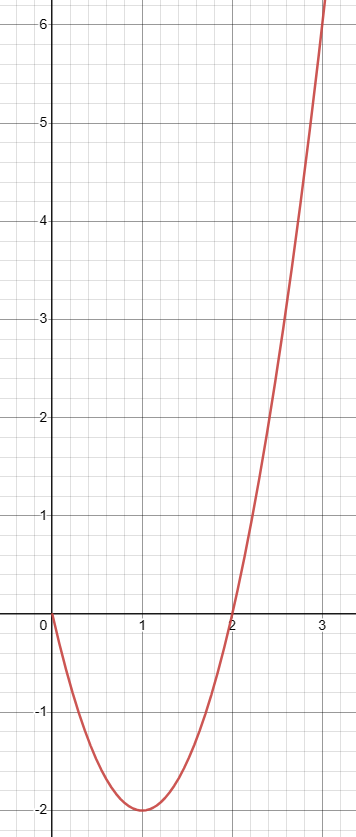
\includegraphics[width=3in]{def_int_Ex.png}
    \hspace{-1in}
    \begin{enumerate}
    \item Compute the right Riemann sum with $n=3$ for the first\\ 3 hours.\\\\\\\\\\\\\\\\\\\\
    \item Sketch the rectangles that correspond to your Riemann sum\\
    Is this an overestimate or underestimate?\\\\
    \item Does your Riemann sum represent a total distance traveled\\ or a displacement(distance from starting point to end point)?\\\\\\
    \item How might you modify your work to approximate the total\\ distance traveled?\\\\\\\\\\\\\\\\\\\\
    \item Express the the displacement and the total distance traveled\\ as definite integrals.
    \end{enumerate}
\end{vwcol} 
\newpage
\begin{enumerate}
    \item Sketch the function $f(x)=6$ on $[-1,5]$. Write the definite integral to compute the area between $f(x)$ and the $x$-axis. Use Geometry to compute the integral exactly.\\\\\\\\\\\\\\\\\\
    \item Sketch the function $g(x)=2x$ on $[-3,4]$. Write the definite integral to compute the area between $g(x)$ and the $x$-axis for (a) $[-3,0]$  (b) $[0,4]$  (c) $[-3,4]$. Use Geometry to compute the integrals exactly (Pay close attention to when the integrals will be negative?).\\\\\\\\\\\\\\\\\\\\\\
    \begin{multicols}{2}
        \item The function $g\left(x\right)$ is graphed to the right.  \\
        
        Use geometry to evaluate $\int_{-3}^{6}g\left(x\right)dx$\\
        
        Hint: the graph from 0 to 2 is a semicircle.
        
        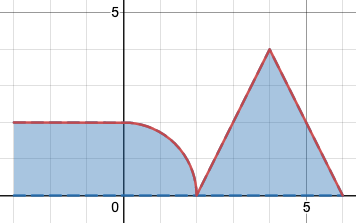
\includegraphics[scale=0.45]{Area1.png}
        \end{multicols}
        
        \vskip 1in
        
        \begin{multicols}{2}
        \item The function $g\left(x\right)$ is graphed to the right.  \\
        
        Use geometry to evaluate $\int_{-3}^{6}g\left(x\right)dx$\\
        
        Hint: the graph from 0 to 2 is a semicircle.
        
        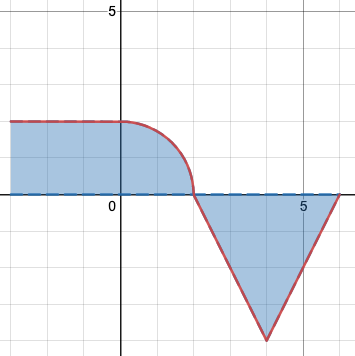
\includegraphics[scale=0.45]{Area2.png}
        \end{multicols}
\end{enumerate}

\end{document}
